\section{The \textbf{TransP-0} integrated design abstraction}
\label{proposed_model}

The \textsc{TransP-0} design abstraction is intended to support both transportation and power system engineers during early project phases in formulating and evaluating different design options quickly. Therefore, transportation and power system properties - both static and dynamic - have to be captured sufficiently precise. On the other hand, the design abstraction should omit unnecessary details to enable frequent design iterations. With these requirements in mind we have developed a candidate design abstraction, which is summarized in Figure~\ref{system_design}. The abstraction comprises various transportation and a power respectively energy subsystem properties as well as subsystem-specific and -spanning constraints and objectives.

\begin{figure}[h!]
	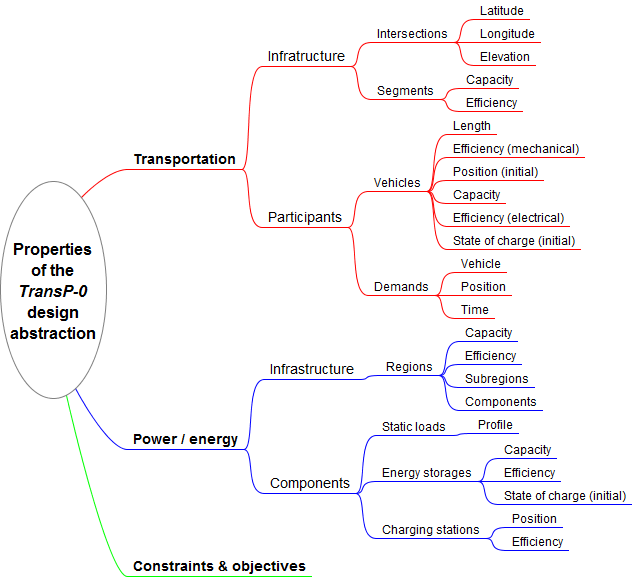
\includegraphics[width=\columnwidth]{./gfx/system_design.png}
	\caption{\textsc{TransP-0} integrated design abstraction comprising various transportation subsystem and power subsystem properties as well as subsystem-specific and -spanning constraints and objectives.}
	\label{system_design}
\end{figure}

In the following, we first describe the design abstraction for the transportation subsystem in Section~\ref{transport} and the power respectively energy subsystem in Section~\ref{energy_system}. Then, we explain the subsystem-specific and -spanning constraints in Section~\ref{constraints} as well as the objectives in Section~\ref{objectives}. 

\subsection{Transportation subsystem}
\label{transport}

The transportation subsystem $TS$ of the integrated design abstraction is modeled as a tuple
\[
	TS = (TSI, TSP) \textrm{,}
\]
where $TSI$ represents the transportation infrastructure (i.e.\ roads and their intersections) and $TSP$ represents the individual traffic participants (i.e.\ passenger cars and goods vehicles). In the following, we describe the the infrastructure design abstraction in Section~\ref{transport_infrastructure} before explaining the participant design abstraction in Section~\ref{participants}.

\subsubsection{Infrastructure}
\label{transport_infrastructure}

The transportation subsystem infrastructure $TSI$ of the transportation subsystem $TS$ is modeled as a tuple
\[
	TSI = (RI, RS) \textrm{,}
\]
where $RI$ represents road intersections and $RS$ represent road segments. Subsequently, we first describe the road intersections in Section~\ref{intersections} before explaining the road segments in Section~\ref{segments}.

\paragraph{Intersections}
\label{intersections}

The road intersections $RI$ of the transportation subsystem infrastructure $TSI$ are modeled - again - as a tuple
\[
	RI = (RIL, RIC) \textrm{,}
\]
where $RIL$ represents a finite set of road intersection labels and $RIC$ represents a mapping from road intersection labels $RIL$ to geometric coordinates
\[
	RIC: RIL \rightarrow \mathbb{R}^3 \mathrm{.}
\]
Note that typically the coordinates are expressed in terms of latitude, longitude, and elevation. However, for simplicity in this work we use Cartesian coordinates instead. Consequently, distances can be computed more easily using the Euclidean metric. Moreover, transformations exist to switch between polar and Cartesian coordinates.

\paragraph{Segments}
\label{segments}

In contrast, the road segments $RS$ of the transportation subsystem infrastructure $TSI$ are modeled as a five-tuple
\[
	RS = (RSL, RSS, RST, RSC, RSE) \textrm{,}
\]
where $RSL$ represents a finite set of road segment labels, $RSS$ and $RST$ represent mappings from road segment labels $RSL$ to their respective source and target road intersection labels $RIL$
\[
	RSS/RST: RSL \rightarrow RIL \textrm{,}
\]
$RSC$ represents a mapping from road segment labels $RSL$ to the number of lanes (i.e.\ the \textit{capacity} of the road segment)
\[
	RSC: RSL \rightarrow \mathbb{N} \textrm{,}
\]
and $RSE$ represents a mapping from road segment labels $RSL$ to their surface material (i.e.\ the \textit{efficiency} of the road segment)
\[
	RSE: RSL \rightarrow \mathbb{R}^+ \textrm{.}
\]
Note that the previous parameters completely determine our road segment model. Consequently, we abstract from a variety of parameters typically considered such as \todo{...}.

Furthermore, we derive the road segment distance $RSD$ as a mapping from road segment labels $RSL$ to distances
\[
	RSD: RSL \rightarrow \mathbb{R}_0^+
\]
and we use the Euclidean metric $E: \mathbb{R}^3 \times \mathbb{R}^3 \rightarrow \mathbb{R}_0^+$ to compute the road segment distance $RSD$ as
\[
	RSD(rsl) = E(RIC(RSS(rsl)), RIC(RST(rsl))) \textrm{.}
\]
Finally, we define road segment positions $RSP$ as tuples of road segment labels $RSL$ and traveled distances
\[
	RSP = \{(rsl, d) \in RSL \times \mathbb{R}_0^+ \mid d \leq RSD(rsl)\} \textrm{.}
\]
We use the road segment positions $RSP$ to locate traffic participants (i.e.\ vehicles) on the transportation subsystem infrastructure $TSI$ as explained in Section~\ref{participants}.

\subsubsection{Participants}
\label{participants}

The transportation subsystem participants $TSP$ of the transportation subsystem $TS$ are modeled - again - as a tuple
\[
	TSP = (V, D) \textrm{,}
\]
where $V$ represents the vehicles and $D$ represents the demands. In the following, we first describe the vehicle design abstraction in Section~\ref{vehicles} before explaining the demand design abstraction in Section~\ref{demands}.

\paragraph{Vehicles}
\label{vehicles}

The vehicles $V$ of the transportation subsystem participants $TSP$ are modeled as seven-tuple
\[
	V = (VL, VS, VME, VP_0, VC, VEE, VSOC_0) \textrm{,}
\]
where $VL$ represents a finite set of vehicle labels, $VS$ represents a mapping from vehicle labels $VL$ to their length (i.e.\ the \textit{size} of the vehicle in road segment direction)
\[
	VS : VL \rightarrow \mathbb{R}^+ \textrm{,}
\]
$VME$ represents a mapping from vehicle labels $VL$ to their mechanical efficiency (i.e.\ a constant ratio for the conversion between electrical and mechanical energy)
\[
	VME : VL \rightarrow \mathbb{R}^+ \textrm{,}
\]
$VP_0$ represents a mapping from vehicle labels $VL$ to their initial road segment positions $RSP$ (see Section~\ref{segments})
\[
	VP_0 : VL \rightarrow RSP \textrm{,}
\]
$VC$ represents a mapping from vehicle labels $VL$ to their battery capacities (i.e.\ the maximum amount of energy that can be stored by the vehicle)
\[
	VC : VL \rightarrow \mathbb{R}^+ \textrm{,}
\]
$VEE$ represents a mapping from vehicle labels $VL$ to their electrical efficiency (i.e.\ a constant ratio for conversion between electrical energy and stored energy)
\[
	VEE : VL \rightarrow \mathbb{R}^+ \textrm{,}
\]
and $VSOC_0$ represents a mapping from vehicle labels $VL$ to their initial state of charge (i.e.\ the amount of energy stored by the vehicle initially)
\[
	VSOC_0 : VL \rightarrow \mathbb{R}^+ \textrm{ such that } VSOC_0(vl) \leq VC(vl) \textrm{.}
\]
Note that again we abstract from many parameters typically considered such as \todo{...}. In particular, we approximate mechanical and electrical efficiencies with constants only.

\todo{State / actions? $RSL^* \times \mathbb{R}_0^+ \Rightarrow VP_{t+1} \times VSOC_{t+1}$}

\paragraph{Demands}
\label{demands}

Finally, the demands $D$ of the transportation subsystem participants $TSP$ are modeled as four-tuple
\[
	D = (DL, DV, DP, DT) \textrm{,}
\]
where $DL$ represents a finite set of demand labels, $DV$ represents a mapping from demand labels $DL$ to vehicle labels $VL$ (i.e.\ the concerned vehicle)
\[
	DV: DL \rightarrow VL \textrm{,}
\]
$DP$ represents a mapping from demand labels $DL$ to road segment positions $RSP$ (i.e.\ where the concerned vehicle is expected to be)
\[
	DP: DL \rightarrow RSP \textrm{,}
\]
and $DT$ represents a mapping from demand labels $DL$ to time points (i.e.\ when the concerned vehicle is expected to be there)
\[
	DT: DL \rightarrow \mathbb{N}^+ \textrm{.}
\]
Note that our abstraction is based on discrete time. However, we do not prescribe the time step resolution.

\subsection{Power / energy subsystem}
\label{energy_system}

The energy subsystem $ES$ of the integrated design abstraction is modeled as a tuple
\[
	ES = (ESI, ESC) \textrm{,}
\]
where $ESI$ represents the energy subsystem infrastructure (determined by the transmission and distribution network) and $ESC$ represents energy subsystem components (i.e.\ the actual producers and consumers). In the following, we first explain the infrastructure in Section~\ref{regions} before describing the components in Section~\ref{components}.

\subsubsection{Infrastructure}
\label{energy_infrastructure}

The energy subsystem infrastructure $ESI$ of the energy subsystem $ES$ is modeled as a one-tuple
\[
	ES = (R) \textrm{,}
\]
where $R$ represents the regions of the energy subsystem infrastructure, which are determined by the voltage levels and transformers of the network. Note that we selected a region model~\cite{Hackenberg2012} over a power flow model~\cite{Dommel1968} to reduce modeling effort and increase computational efficiency. In the following, we describe the regions in Section~\ref{regions}.

\paragraph{Regions}
\label{regions}

The regions $R$ of the energy subsystem infrastructure $ESI$ are modeled as a five-tuple
\[
	R = (RL, RC, RE, RSR, RSC) \textrm{,}
\]
where $RL$ represents a finite set of region labels, $RC$ represents a mapping from region labels $RL$ to region \textit{capacities} (i.e.\ the maximum amount of energy that can flow through that region in a predefined time interval)
\[
	RC: RL \rightarrow \mathbb{R}^+ \textrm{,}
\]
$RE$ represents a mapping from region labels $RL$ to region \textit{efficiencies} (i.e.\ a constant factor determining the energy that is lost while flowing through that region)
\[
	RE: RL \rightarrow \mathbb{R}^+ \textrm{,}
\]
$RSR$ represents a mapping from region labels $RL$ to a subset of region labels (i.e.\ the labels of the respective subregions)
\[
	RSR: RL \rightarrow \mathcal{P}(RL) \textrm{,}
\]
and $RSC$ reprsents a mapping from region labels $RL$ to a subset of component labels (i.e.\ the labels of the components connected to that region; see Section~\ref{components})
\[
	RSC: RL \rightarrow \mathcal{P}(CL) \textrm{.}
\]
Note that regions and components must be assigned to at most one parent region. Consequently, our region model represents the energy system as a tree structure. The nodes of the tree represent \textit{subnetworks} with distinct voltage levels. The edges of the tree represent \textit{transformers} connecting the subnetworks instead. Consequently, the region model can be derived easily from existing network topologies.

\todo{State? $RB_t$}

\subsubsection{Components}
\label{components}

The energy subsystem components $ESC$ of the energy subsystem $ES$ is modeled as a three-tuple
\[
	ESC = (SL, ES, CS) \textrm{,}
\]
where $SL$ represents the static (i.e.\ uncontrollable) energy loads, $ES$ represents the stationary energy storages, and $CS$ represents the charging stations for the electric vehicles (see Section~\ref{vehicles}). In the following, we first explain the static load design abstraction in Section~\ref{static_loads}, before describing the energy storage design abstraction in Section~\ref{energy_storages} and presenting the charging station design abstraction in Section~\ref{charging_stations}.

\paragraph{Static loads}
\label{static_loads}

The static loads $SL$ of the energy subsystem components $ESC$ are modeled as tuple
\[
	SL = (SLL, SLP) \textrm{,}
\]
where $SLL$ represents a finite set of static load labels and $SLP$ represents a mapping from static load labels $SLL$ to static load profiles
\[
	SLP: SLL \rightarrow (\mathbb{N} \rightarrow \mathbb{R}) \textrm{.}
\]
Note that a static load profile associates a numeric load to each discrete time step. Hereby positive numbers represent energy production and negative loads represent energy consumption. Consequently, static loads can be used to model everything from home appliances to solar panels to conventional power generators. In particular, we assume such loads to be uncontrollable in our design abstraction.

\todo{State?}

\paragraph{Energy storages}
\label{energy_storages}

Then, the energy storages $ES$ of the energy subsystem components $ESC$ are modeled as a four-tuple
\[
	ES = (ESL, ESCA, ESE, ESS_0) \textrm{,}
\]
where $ESL$ represent a finite set of energy storage labels, $ESCA$ represents a mapping from energy storage labels $ESL$ to energy storage \textit{capacities} (i.e.\ the maximum amount of energy that can be stored)
\[
	ESCA: ESL \rightarrow \mathbb{R}^+ \textrm{,}
\]
$ESE$ represents a mapping from energy storage labels $ESL$ to energy storage \textit{efficiencies} (i.e.\ a constant factor between inflow energy and stored energy)
\[
	ESE: ESL \rightarrow \mathbb{R}^+ \textrm{,}
\]
and $ESS_0$ represents a mapping from energy storage labels $ESL$ to initial \textit{state of charges} (i.e.\ the amount of energy stored initially)
\[
	ESS_0: ESL \rightarrow \mathbb{R}_0^+ \textrm{ such that } ESS_0(esl) \leq ESCA(esl)
\]
Note that the energy storage model is analogous to the electric vehicle model present in Section~\ref{vehicles}. Only, electric vehicles also include mechanical properties.

\todo{State? Action? $ESLO_{t+1} \rightarrow ESS_{t+1}$}

\paragraph{Charging stations}
\label{charging_stations}

Finally, the charging stations $CS$ of the energy subsystem components $ESC$ are modeled as a three-tuple
\[
	CS = (CSL, CSP, CSE) \textrm{,}
\]
where $CSL$ represents a finite set of charging station labels, $CSP$ represents a mapping from charging station labels $CSL$ to road segment labels $RSL$ with zero road segment distance
\[
	CSP: CSL \rightarrow RSL \textrm{ such that } RSD(CSP(csl)) = 0 \textrm{,}
\]
and $CSE$ represents a mapping from charging station labels $CSL$ to charging station efficiencies (i.e.\ the energy lost while flowing through the charging station)
\[
	CSE: CSL \rightarrow \mathbb{R}^+ \textrm{.}
\]
Note that in particular the charging station position mapping $CSP$ defines the connections between the transportation subsystem and the power subsystem.

\todo{State?}

\subsection{Constraints}
\label{constraints}

In principle, one can define arbitrary constraints over the static and dynamic system properties presented in the previous sections. In particular, we believe that such constraints might arise from design decisions made by transportation and energy system engineers. Hence, we do not want to prescribe the constraints. Rather, we provide two basic constraints which we believe to be part of any integrated system design. The first constraint makes sure that the road segment capacities $RSC$ (i.e.\ the number of lanes) of the transportation subsystem infrastructure $TSI$ are not exceeded (see Section~\ref{collisions}). The second constraint makes sure that the region capacities $RC$ of the energy subsystem infrastructure $ESI$ are not exceeded (see Section~\ref{capacities}).

\subsubsection{Segment capacities}
\label{collisions}

TODO

%Overlapping vehicle pairs $OVP : \mathbb{VS} \rightarrow V \times V$
%\[
%OVP(VS) = \{(v_1, v_2) \in V \times V \mid
%\]
%\[
%((rs_1,rd_1),\cdot) \in VS(v_1), ((rs_2,rd_2),\cdot) \in VS(v_2) :
%\]
%\[
%rs_1 = rs_2 \wedge (|rd_1 - rd_2| < VL(v_1) / 2
%\]
%\[
%\vee
%\]
%\[
%|rd_1 - rd_2| < VL(v_2) / 2)\}
%\]
%Overlapping vehicle sets $OVS : \mathbb{VS} \times V \rightarrow \mathcal{P}(V)$
%\[
%OVS(VS,v) = \{v' \in V \mid (v, v') \in OVP(VS)\}
%\]
%Collision property $CV : \mathbb{VS} \rightarrow \mathbb{B}$
%\[
%CV(VS) \Leftrightarrow \exists v \in V :
%\]
%\[
%|OVS(VS, v)| > RSL(rs) \text{ with } ((rs,\cdot),\cdot) = VS(v)
%\]

\subsubsection{Region capacities}
\label{capacities}

TODO

\subsection{Objectives}
\label{objectives}

TODO

%The objective function in our model is made up from multiple cost factors, which we describe subsequently:
%
%\begin{table}[h!]
%	\centering
%	\renewcommand{\arraystretch}{1.3}
%	\begin{tabularx}{\columnwidth}{|Y|Y|}
%		\hline
%		
%		\textbf{Objective} & \textbf{Behavior} \\
%		
%		\hline
%		
%		Energy-efficiency &
%		The energy-efficiency cost function measures a vehicle's current state of charge in relation to it's maximum state of charge. \\
%		
%		\hline
%		
%		Time &
%		The time cost function counts the number of steps for a vehicle to reach it's destination, when a driving decision has been made. \\
%		
%		\hline
%		
%		SoC &
%		Measures the current state of charge of a traffic participants battery. Increases when a traffic participants departure time nears. \\
%		
%		\hline
%		
%		Derivation from arrival time &
%		Measures the derivation from a traffic participants planned arrival time. \\
%		
%		\hline
%		
%		Derivation from destination &
%		Measures the derivation from the position of the destination road segment. \\
%		
%		\hline			
%	\end{tabularx}
%	\caption{Individual vehicle objectives and description.}
%	\label{figure:objectives}
%\end{table}
%
%Costs are aggregated hierarchically within the given component structure by the root component from each contained sub component. Our methodology allows for each component to implement it's own set of cost functions and constraints. 
%
%\todo{Move into the model or the demonstration?}
%
%The objective function for individual traffic participants in our model is made up from multiple cost factors, which we describe subsequently: